\section{Examples, interpretation, and exact testing thresholds}
\label{sec:examples}

\subsection{A binary four-dimensional example}

Take $\OO=\mathbb Z_2$ and $g=2$. Then $N=2$, $\alpha_g=4/5$, and
\[
 h_2(A)=\frac45\sum_{r=0}^{v_2(1-\det A)}2^{-r}.
\]
The likelihoods at valuations $0,1,2,3$ are respectively
$4/5,6/5,7/5,3/2$, tending to $8/5$ as the defect tends to zero.
They cross one exactly once: between valuation zero and valuation one.

Under the independent-entry law, $\det A$ is odd with probability
$3/8$. Under the symplectic-corner law it is odd with probability
$1/2$. Thus
\[
 \TV(\mu_e,\nu_e)=\frac18,
 \qquad \text{optimal equal-prior success probability}=\frac9{16},
\]
whether the observer sees the matrix modulo $2$, modulo $2^{1000}$,
or as a full $2$-adic matrix. The optimal test declares the
symplectic-corner model exactly when the determinant is odd.

Nevertheless the conditional laws inside that odd-determinant residue
event are different. The law obtained by keeping only the exact
modulo-$2$ distribution and completing uniformly differs from the
true law by $1/40$. Keeping $k$ exact digits instead gives the error
\[
 \TV(\mu_\infty,\widetilde\mu_{k,\infty})
 =\frac{1}{10\cdot4^k}.
\]
The distinction is between preserving the best equal-prior test against
independent entries and preserving the entire probability law.
The first happens after one digit; the second does not.

\begin{figure}[tbp]
\centering
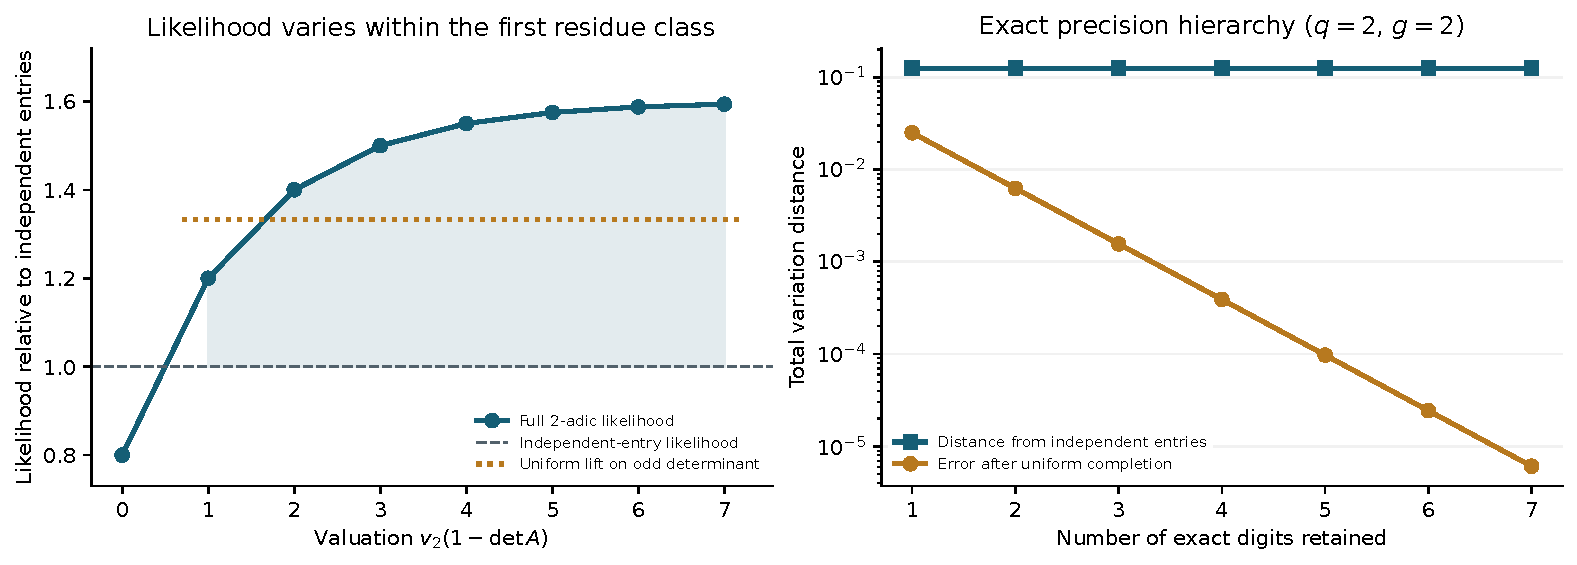
\includegraphics[width=\textwidth]{figures/precision_laws.pdf}
\caption{Left: the complete-ring likelihood for $q=2,g=2$ changes with
the determinant-defect valuation but remains above one for every positive
valuation. Right: the exact uniform-completion error decreases with retained
precision, while the distance from independent entries stays fixed.
All plotted values are evaluations of proved formulas.}
\label{fig:precision}
\end{figure}

\subsection{The complete optimal-threshold curve}

The exact density also describes tests with unequal costs or unequal
prior probabilities. Put $E_r=\{A:1-\det A\in\pi^r\OO\}$ for $r\ge1$
and $\beta_q=(q^2-1)/q^3$. Under the two complete-ring laws,
\begin{align}
 \nu_\infty(E_r)&=\beta_q q^{-(r-1)},\label{eq:roc-uniform}\\
 \mu_\infty(E_r)&=\beta_q q^{-(r-1)}
 \frac{(1-q^{-N})\sum_{j=0}^{r-1}q^{-(N-1)j}
       +q^{-(N-1)r}}{1-q^{-2g}}.\label{eq:roc-symplectic}
\end{align}
Indeed, the first formula follows by varying a unit pivot, and the
second is the finite-$r$ likelihood on the zero-defect class multiplied
by its uniform probability. Because the complete-ring likelihood is
strictly increasing with the valuation, likelihood-threshold tests
are exactly these congruence events, together with the empty or full
event and possible randomization on a level set.

For $q=2,g=2$, the first three threshold points
$(\nu(E_r),\mu(E_r))$ are
\[
 \left(\frac38,\frac12\right),\qquad
 \left(\frac3{16},\frac{11}{40}\right),\qquad
 \left(\frac3{32},\frac{23}{160}\right).
\]
Their largest vertical difference is the first, namely $1/8$.
Different likelihood thresholds can favor the later points; the
one-digit result is therefore not a claim of statistical sufficiency
for every decision problem.

\subsection{Cokernels and dimensions}

In the same binary example a Haar independent matrix has trivial
cokernel with probability $3/8$. The symplectic corner has trivial
cokernel with probability $1/2$. Every nontrivial type has probability
$4/5$ of its independent-model probability. For example,
\[
 \Pr\bigl(\coker M\simeq\mathbb Z_2/(2)\bigr)=\frac9{40},\qquad
 \Pr\bigl(\coker M\simeq(\mathbb Z_2/(2))^2\bigr)=\frac3{160}.
\]
After conditioning on nontrivial cokernel, the factor cancels and the
two entire module distributions agree exactly.

\begin{center}
\begin{tabular}{@{}cccc@{}}
\toprule
$q$ & $g$ & $\TV(\mu_e,\nu_e)$, all $e$ & $\TV(\mu_e,\widetilde\mu_{1,e})$, $e\ge2$\\
\midrule
$2$ & $2$ & $1/8$ & $1/40$\\
$2$ & $3$ & $5/168$ & $1/672$\\
$3$ & $2$ & $19/270$ & $1/135$\\
$3$ & $3$ & $19/2457$ & $2/22113$\\
\bottomrule
\end{tabular}
\end{center}
The exact distances depend on the residue cardinality, the symplectic
dimensions, and the precision in the specified way. They do not
depend on a ramification index or on whether the fraction field has
characteristic zero. This follows from the proofs and is corroborated
by the different finite-ring models tested below.
